\section{Introduction}

This is the first mandatory assignment for the course SIGB F2013. In
this assignment we'll implement a simple gaze tracker. This will be done
in the programming language python with help from the opencv and numpy
libraries.

This report is an attempt to document what has been done to make this
gaze tracker.

The basic structure for each section will be a short introduction of the
goal of the section, followed by the theory behind our approach ending
with a description of our actual implementation with visual aids used
for documentation. Additionally we will accompany the report with
captured videos demonstrating the usage of the eye tracker

\begin{figure}[htbp]
\centering
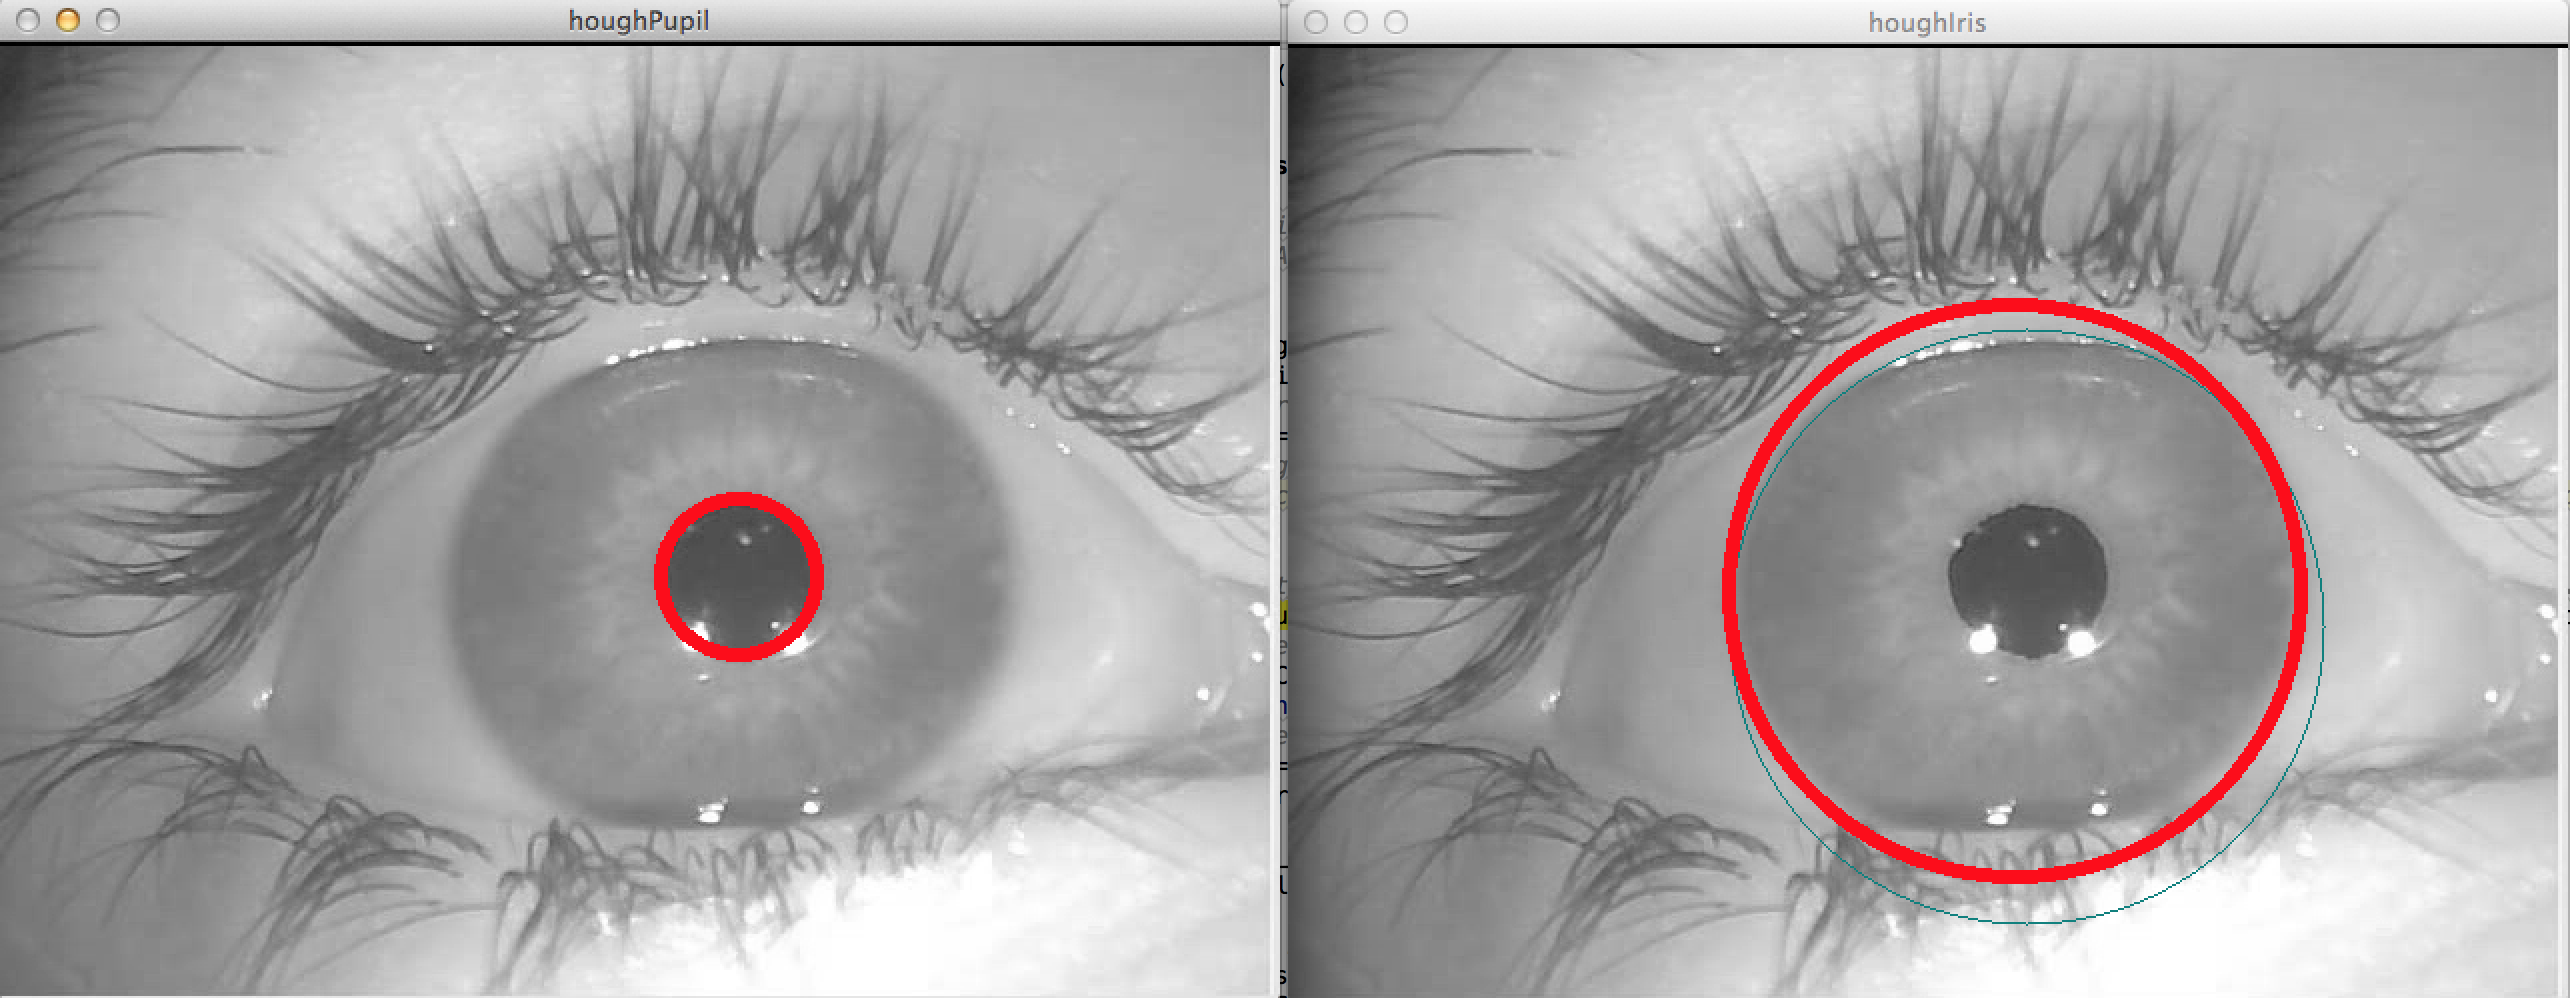
\includegraphics{pics/houghtransform.png}
\caption{Eye located with hough}
\end{figure}

\section{Pupil detection}

\subsection{Overall rationale and theory}

The eye consists of several distinct features such as pupil, iris,
limbus and sclera. The position of these can aid in correctly
determining the gaze. Detecting these features is therefore a good
starting for a gaze tracker implementation, but it poses some challanges
in correctly identifying each component, and filtering away noise.

Of these features one of the easiest to recognize is the pupil, as it is
the darkest part of the eye. Furthermore it's good starting point, as it
is surrounded by the other eye components. The challenges/noise in
locating the pupil is mostly due to glints/reflections of light.

As mentioned, the pupil is the darkest part of the eye. Therefore a good
way to find is to find an intensity value which can seperate it from the
background. This is called thresholding, and will be explained in the
following sections. Following these is a description of a method
automatically setting this threshold value, clustering.

\subsection{Thresholding}

Thresholding is a form of point processing used for seperating areas of
an image based on intensity in these areas. The desired end result of
this method is a binary image with the foreground (object) in one color
and the background (everything else) in a different color. This is
usually black and white respectively. This will effectively seperate the
foreground from the background for us, leaving us with only the
contours. In that sense we loose information and granularity in the
image, but since we're only interested in position we haven't lost
anything important.

\subsubsection{Theory}

As with all point processing methods the basic theory behind
thresholding is applying a calculation to every pixel in the image,
effectively changing the value of that pixel. We know that the end
result is a binary image, following this each pixel will be transformed
into one of two values. We've so far operated on byte images so the max
value is 255 and the min value is of course 0. For clarity we will
assign each pixel either the min or the max value. Thus thresholding can
be expressed as the following with T being the assigned Threshold value
and f being the function applied to each pixel:

if f$(x,y) \leq T \quad then \, g$(x,y) = 0 \quad and \quad if
f$(x,y) < T \quad then \, g$(x,y) = 255

Performing these operations will leave us with an image where only the
contours are visible. We can then analyse the properties of these
contours to find which one is most likely to be a pupil

\subsubsection{Our implementation}

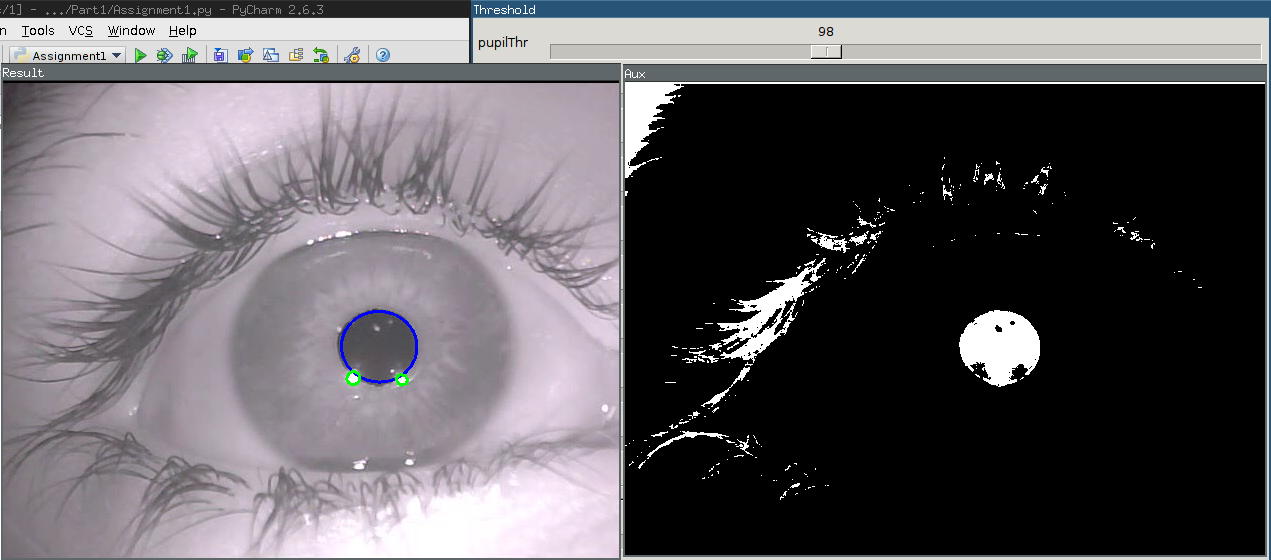
\includegraphics{pics/threshold_good.png}
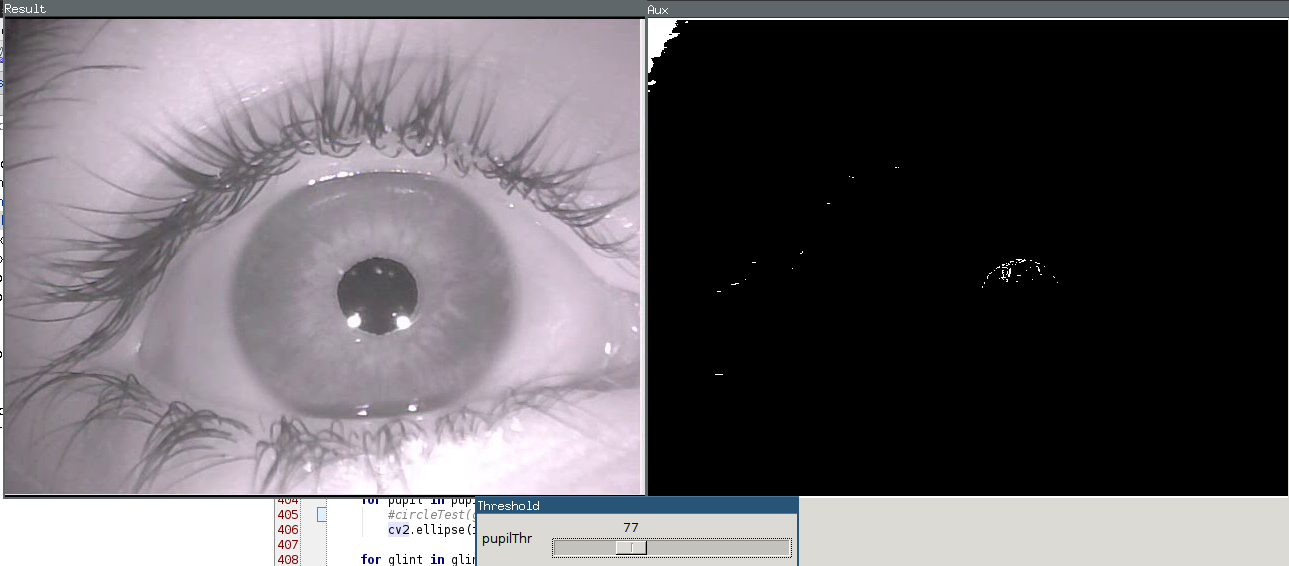
\includegraphics{pics/threshold_low.png}
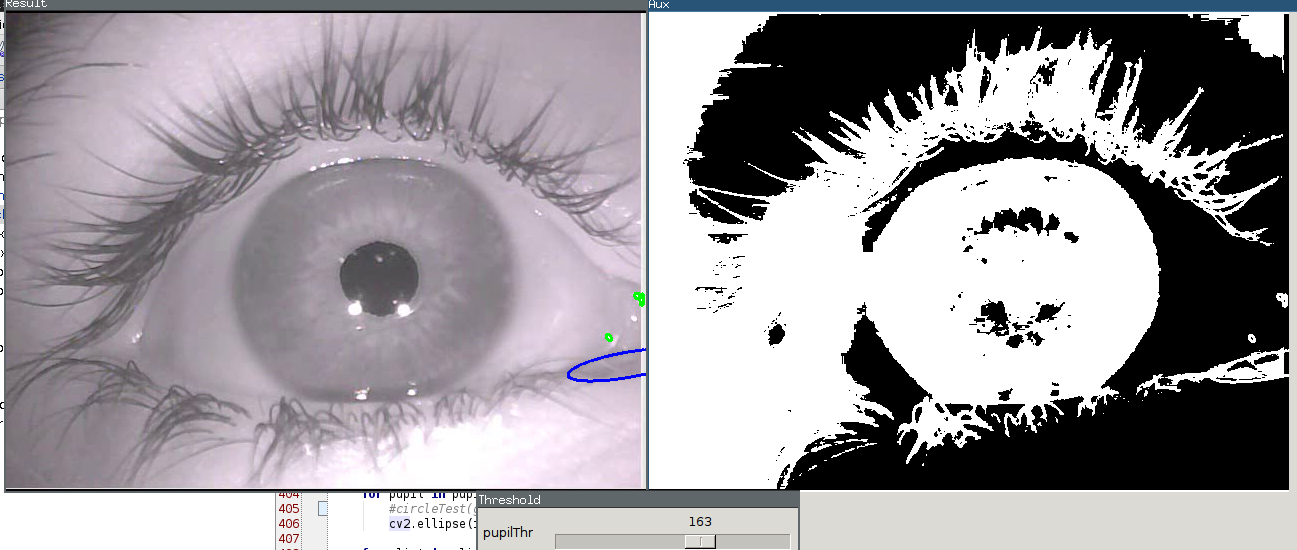
\includegraphics{pics/threshold_high.png}
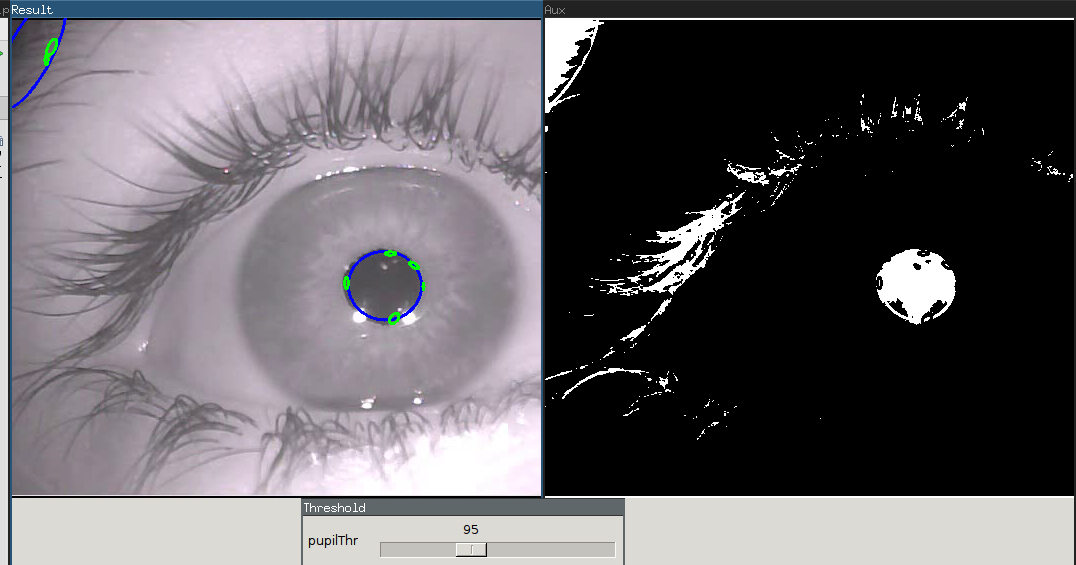
\includegraphics{pics/threshold_contours.png}

\subsection{K-means clustering}

In this section it will be demonstrated how a form of machine learning
is applied in order to perform supervised classification in order to
semi-automatically set a proper thresholding value

Clustering is the practice of grouping a set of elements into several
smaller groups of elements with similar features. It has a wide range of
applications within datamining and different types of analysis.
Obviously what will be demonstrated here is it's use within image
analysis. Clustering isn't a specific algorithm. Rather it's the task we
wish to perform in order to achieve our goal. In this assignment we've
used the k-means algorithm for this

K-means is a clustering algorithm which can group a number of
observations/data points into k number of clusters based on their
nearest mean value.

The properties of the k-means algorithm (k groups based on mean
intensity) combined with an existing knowledge of the properties of the
eye(the pupil is the darkest part) makes it possible to use k-means for
setting a threshold value automatically

\subsubsection{Theory}

The basic idea behind k-means clustering is to iteratively run through a
dataset assigning points in their correct cluster based on previously
selected values. Initially k points a selected and denoted as a center
for it's cluster, c\_1, \ldots{}, c\_k. These points can be selected on
random or based on some guessed distribution. On each run through the
dataset every points is examined. For each point the closest c is found,
and the point is marked as to belong to this cluster. Once all points
have been examined and placed in a cluster, the mean value of each
cluster is calculated as c\_i\_val. Compare the mean value for the
cluster with the previously recorded value of c\_i\_val. If it has
changed, another run through is performed. This continues until a
desired level of precision is achieved or amount of runs have taken
place

When we have done this we have k different threshold values to choose
from, given our knowledge of the pupil, we will choose the one with the
lowest mean value (c\_i\_val).

\subsubsection{Our implementation}

There are a couple of possible caveats for this approach. Firstly there
is an element of uncertainty in exactly how the clusters will be
distributed. We need therefore to have a high enough k value to be sure
to get the right cluster. There is also some uncertainty about whether
the pupil always belongs to the darkest cluster. If for instance our
k-value is too high, and there exists a darker region in the image (dark
spot on the skin for instance) then the value of this cluster will be
chosen as a threshold value, and we might miss the pupil

Through trials it was found that 8 is a good value for k
